\documentclass{article}
\usepackage{tikz}
\usetikzlibrary{positioning}
\usepackage{listings}
\lstset{
  basicstyle=\ttfamily\small,
  breaklines=true,
  frame=single
}

\title{MapReduce Word Count}
\author{Nguyen Viet Khoa}
\date{\today}

\begin{document}

\maketitle

\section{Why the Chosen MapReduce Implementation}
I chose a pure Python simulation of MapReduce using built-in functions like \texttt{map}, \texttt{reduce}, and \texttt{defaultdict} for grouping. This avoids dependencies on external frameworks like Hadoop (which requires setup) or libraries like mrjob (not available). It's educational, lightweight, and runs locally without a cluster, making it ideal for demonstration while illustrating core concepts: map, shuffle/sort, reduce.

\section{How Mapper and Reducer Work}
The Mapper takes text chunks, extracts words using regex, and emits (word, 1) pairs. The shuffle/sort phase groups and sorts these by key. The Reducer sums counts for each word.

\begin{figure}[h]
\centering
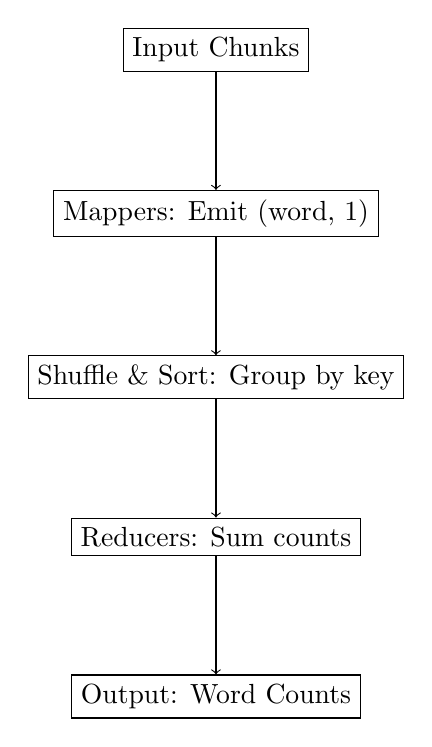
\begin{tikzpicture}
  \node[draw, rectangle] (input) {Input Chunks};
  \node[draw, rectangle, below=of input, yshift=-0.5cm] (map) {Mappers: Emit (word, 1)};
  \node[draw, rectangle, below=of map, yshift=-0.5cm] (shuffle) {Shuffle \& Sort: Group by key};
  \node[draw, rectangle, below=of shuffle, yshift=-0.5cm] (reduce) {Reducers: Sum counts};
  \node[draw, rectangle, below=of reduce, yshift=-0.5cm] (output) {Output: Word Counts};
  \draw[->] (input.south) -- (map.north);
  \draw[->] (map.south) -- (shuffle.north);
  \draw[->] (shuffle.south) -- (reduce.north);
  \draw[->] (reduce.south) -- (output.north);
\end{tikzpicture}
\caption{Mapper and Reducer Workflow}
\label{fig:workflow}
\end{figure}

\section{Who Does What}
\begin{itemize}
  \item \textbf{Mapper}: Processes input chunks, tokenizes into words, and outputs key-value pairs (word, 1) for each occurrence.
  \item \textbf{Shuffle/Sort}: Groups all pairs by key (word) and sorts the keys, preparing for reduction (handled by \texttt{defaultdict} and \texttt{sorted}).
  \item \textbf{Reducer}: Aggregates values for each key by summing the list of 1s, producing the final count.
  \item \textbf{Main Function}: Splits input into chunks, orchestrates map/shuffle/reduce phases, and collects results into a dictionary.
\end{itemize}

\end{document}